%%% UNIT 4
{
\setbeamertemplate{headline}{}
\setbeamertemplate{footline}{
  \begin{beamercolorbox}[wd=\paperwidth,ht=2.2ex,dp=1.5ex]{palette quaternary}
  \end{beamercolorbox}
  }
\begin{frame}[noframenumbering]
\frametitle{\DB{\huge{\textbf{$\blacksquare$ Unit 4}}}}
\myPause
 \begin{itemize}
 \item[] \LARGE{\MB{System responses}}
 \item[] \vspace{-1mm}\LARGE{\MB{Formalising requirements}}
 \item[] \vspace{-1mm}\LARGE{\MB{The control loop}}
 \item[] \vspace{-1mm}\LARGE{\MB{Direct synthesis -- PIDs appearing on the horizon...}}
 \item[] \vspace{-1mm}\LARGE{\MB{Conclusions and discussion}}
 \end{itemize}
\end{frame}
}

\part{}

\section{System responses}
\subsection{}

\begin{frame}\mccz
\frametitleTC{Foreword}
\framesubtitleTC{}
\myPause
 \begin{columns}
  \column[T]{0.35\textwidth}
   \only<2->{\centering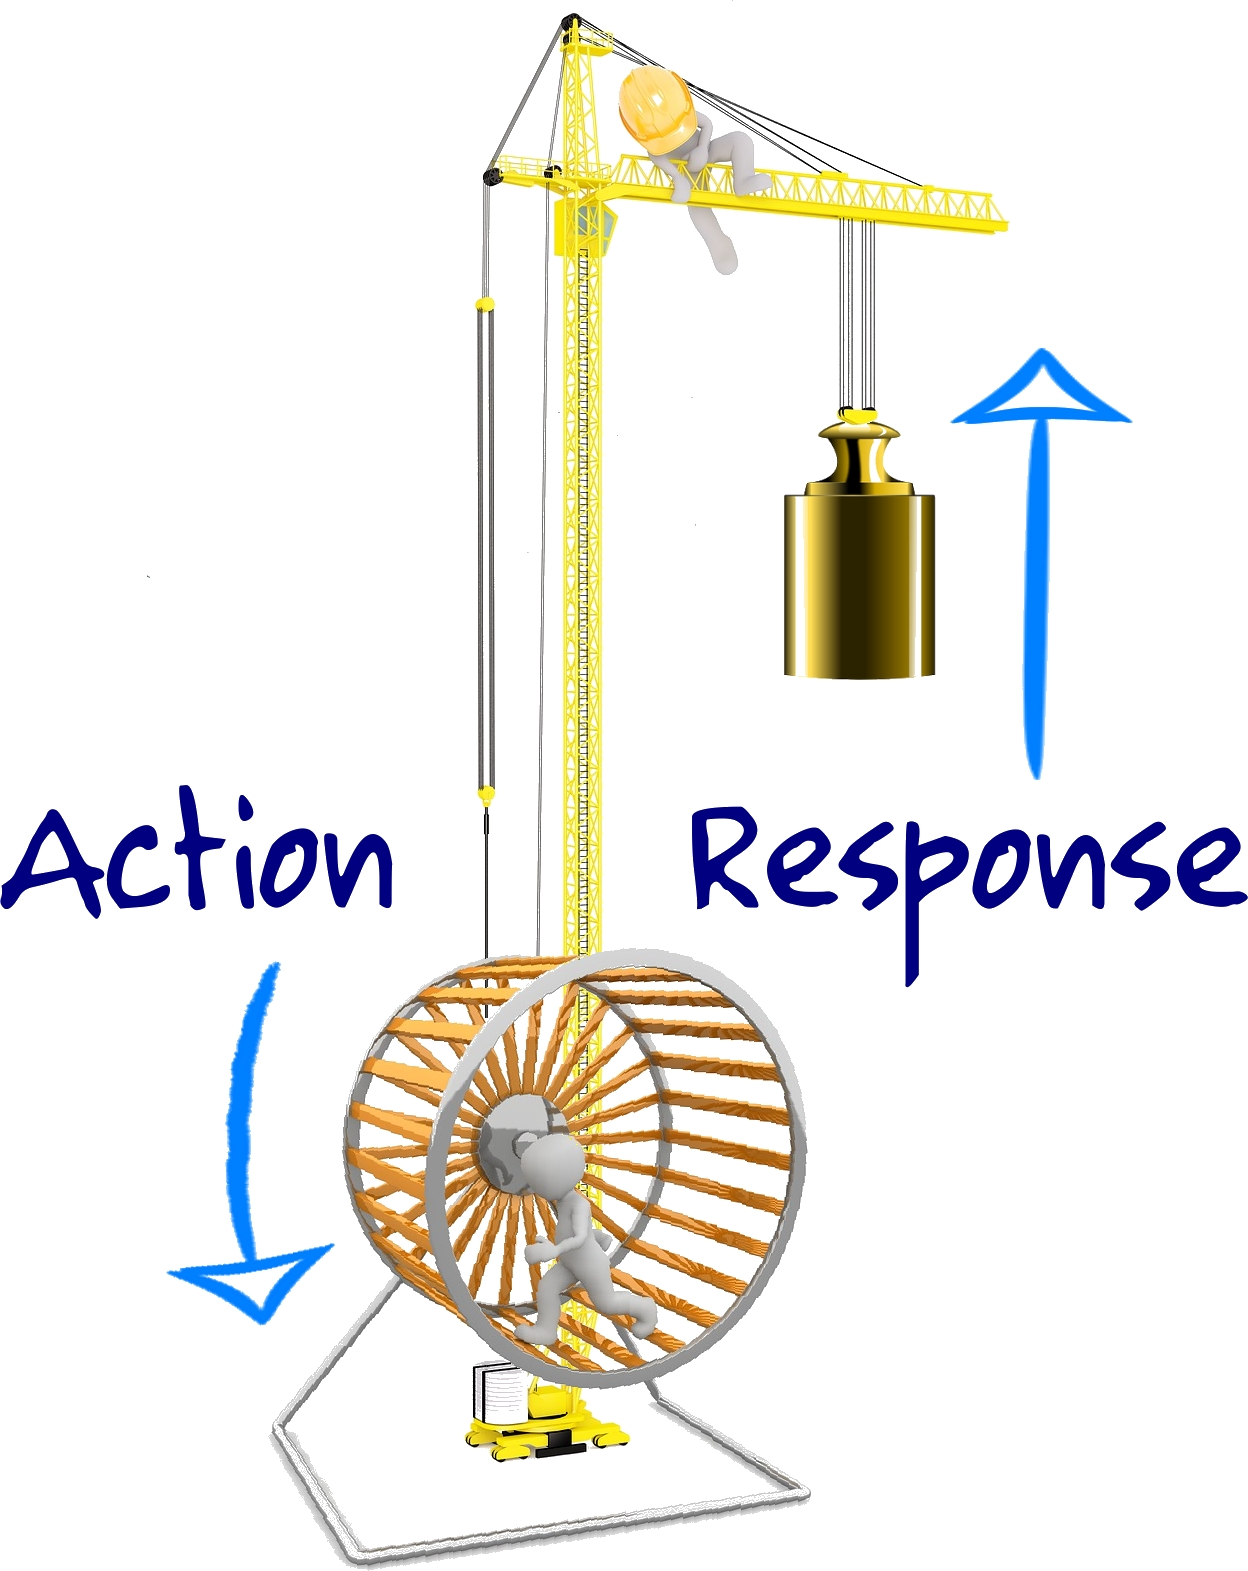
\includegraphics[height=6cm]{./Unit-04/img/response-intro_cc0.jpg}}\myPause%
  \column[T]{0.65\textwidth}
   \begin{itemize}[<+-| alert@+>]
   \item We know how to describe a (DT LTI) dynamic system
         \begin{itemize}[<+-| alert@+>]
         \item in the state space with $(A,b,c,d)$
         \item and with a transfer function $G(z)$.
         \end{itemize}
   \item But how do these descriptions relate to the way\\
         the system responds to a certain \emph{stimulus}?
   \item Specifically for our purpose, can we somehow\\
         relate a transfer function to its\\
         \TC{time (domain) responses}?
   \item \vspace{3mm} Of course we can.
   \item Let us see first how and then why.
   \end{itemize}
 \end{columns}
\end{frame}

\begin{frame}
\frametitleTC{Foreword}
\framesubtitleTC{An introductory case}
\myPause
 \begin{itemize}[<+-| alert@+>]
 \item We showed that as long as a system has only real eigenvalues, its transfer function can be
       expressed as sum/product of elementary first order terms in the form
       \begin{displaymath}
        g(z) = \frac{\mu}{z-p}
       \end{displaymath}
 \item NOTE: if all eigenvalues are distinct, a sum (no products) of terms\\
       like the above suffices.
 \item Given the linearity of the system, responses will sum together the\\
       same way as elementary terms in the transfer function do.
 \item We therefore start by analysing the responses of $g(z)$ above\\
       to a unit impulse and a unit step.
 \item We deal with TI systems, hence in the following everything starts\\
       at $k=0$.
 \end{itemize}
\end{frame}

\begin{frame}
\frametitleTC{An introductory case}
\framesubtitleTC{Impulse response of $g(z)$}
\myPause
 \begin{itemize}[<+-| alert@+>]
 \item Recalling the meaning of $z$, $g(z)$ in the time domain means
       \begin{displaymath}
        y(k) = p y(k-1) + \mu u(k-1).
       \end{displaymath}
 \item Set now $u(k)=imp(k)$, i.e., the sequence $\{1,0,0,0,\ldots\}$. We assume no action on the system
       before $k=0$, consistently with the definition of impulse. We also assume the system at rest, otherwise
       there is free motion and we don not see ONLY the response to $u$, hence $y=0$ for $k<0$.
 \item This said, we get
       {\small
       \begin{displaymath}
        \begin{array}{lclclclclcl}
         y(0) &=& p y(-1) + \mu u(-1) &=& p \cdot 0     + \mu \cdot 0 &=& 0       \\
         y(1) &=& p y(0)  + \mu u(0)  &=& p \cdot 0     + \mu \cdot 1 &=& \mu     \\
         y(2) &=& p y(1)  + \mu u(1)  &=& p \cdot \mu   + \mu \cdot 0 &=& \mu p   \\
         y(3) &=& p y(2)  + \mu u(2)  &=& p \cdot \mu p + \mu \cdot 0 &=& \mu p^2 \\
         \ldots
        \end{array}
       \end{displaymath}
       }
 \item \vspace{-4mm}i.e., the sequence $\{0,\mu,\mu p,\mu p^2,\mu p^3,\ldots\}$.
 \end{itemize}
\end{frame}

\begin{frame}[fragile]
\frametitleTC{An introductory case}
\framesubtitleTC{Impulse response of $g(z)$}
\myPause
 \begin{itemize}[<+-| alert@+>]
 \item Summarising, the impulse response of $g(z)$ is
       \begin{displaymath}
        y(k) = \begin{cases}
                0           & k=0 \\
                \mu p^{k-1} & k>0
               \end{cases}
       \end{displaymath}
 \item Let us compute and plot this response with Scilab:
       {\small
       \begin{verbatim}
 g   = syslin('d',1/(%z-0.5)); // define transfer function ('d' means DT)
 gss = tf2ss(g);               // convert to state space for dsimul
 u   = [1,0,0,0,0,0,0,0,0,0];  // impulse sequence (10 samples)
 y   = dsimul(gss,u);          // compute response
 plot(y,'.');                  // plot (as dots)
       \end{verbatim}
       }
 \item Try different values of $\mu$ and $p$, and comment on the results.
 \end{itemize}
\end{frame}

\begin{frame}
\frametitleTC{An introductory case}
\framesubtitleTC{Impulse response of $g(z)$ -- general remarks}
\myPause
 \begin{itemize}[<+-| alert@+>]
 \item The pole $p$ governs stability as we already know.
 \item For $p=0$ the system is a pure one-step delay.
 \item For $0<p<1$ the response converges monotonically, for $-1<p<0$ oscillating.
 \item In both cases, $p$ governs the convergence speed.
 \item For $p=1$ the response is constant, for $p=-1$ a sustained oscillation\\
       (in both cases for $k>0$, obviously).
 \item Parameter $\mu$ acts as a (signed) scale factor.
 \end{itemize}
\end{frame}

\begin{frame}
\frametitleTC{An introductory case}
\framesubtitleTC{Step response of $g(z)$}
\myPause
 \begin{itemize}[<+-| alert@+>]
 \item Set $u(k)=step(k)$, i.e., the sequence $\{1,1,1,1,\ldots\}$.
 \item We can verify that this yields the response
       \begin{displaymath}
        y(k) = \frac{\mu}{1-p}(1-p^k)
       \end{displaymath}
 \item To this end, we observe that with $\mu=1-p$ we get $y(k) = 1-p^k$:
       {\scriptsize
       \begin{displaymath}
        \begin{array}{lclclclclcl}
         y(0) &=& p \cdot 0       + (1-p) \cdot 0 & &           &=& 0     \\
         y(1) &=& p \cdot 0       + (1-p) \cdot 1 & &           &=& 1-p   \\
         y(2) &=& p \cdot (1-p)   + (1-p) \cdot 1 &=& p-p^2+1-p &=& 1-p^2 \\
         y(3) &=& p \cdot (1-p^2) + (1-p) \cdot 1 &=& p-p^3+1-p &=& 1-p^3 \\
         y(4) &=& p \cdot (1-p^3) + (1-p) \cdot 1 &=& p-p^4+1-p &=& 1-p^4 \\
         y(5) &=& p \cdot (1-p^4) + (1-p) \cdot 1 &=& p-p^5+1-p &=& 1-p^5 \\
         \ldots
        \end{array}
       \end{displaymath}
       }
 \item \vspace{-4mm}Hence a generic $\mu$ scales $y$ to give the result above.
 \end{itemize}
\end{frame}

\begin{frame}[fragile]
\frametitleTC{An introductory case}
\framesubtitleTC{Step response of $g(z)$}
\myPause
 \begin{itemize}[<+-| alert@+>]

 \item Also for the step response case, let us compute and plot some examples with Scilab:
       {\small
       \begin{verbatim}
 g   = syslin('d',1/(%z-0.5)); // define transfer function ('d' means DT)
 gss = tf2ss(g);               // convert to state space for dsimul
 u   = ones(1,10)              // step sequence (a row of 10 samples)
 y   = dsimul(gss,u);          // compute response
 plot(y,'.');                  // plot (as dots)
       \end{verbatim}
       }
 \item Try again different values of $\mu$ and $p$, and comment on the results.
 \end{itemize}
\end{frame}

\begin{frame}
\frametitleTC{An introductory case}
\framesubtitleTC{Step response of $g(z)$ -- general remarks}
\myPause
 \begin{itemize}[<+-| alert@+>]
 \item The pole $p$ governs stability as we already know.
 \item For $p=0$ the system is a pure one-step delay.
 \item For $0<p<1$ the response converges monotonically, for $-1<p<0$ oscillating.
 \item In both cases, $p$ governs the convergence speed.
 \item For $p=1$ the response is a diverging ramp, for $p=-1$ a sustained oscillation.
 \item If $y(k)$ converges, it does so to the value
       \begin{displaymath}
        \frac{\mu}{1-p} = g(1)
       \end{displaymath}
       that is called the \TC{gain} of the transfer function.
 \item Hence for an asymptotically stable $g(z)$, if for $k\rightarrow\infty$ $u(k)\rightarrow\overline{u}$,\\
       then $y(k)\rightarrow g(1)\overline{u}$.
 \end{itemize}
\end{frame}

\begin{frame}
\frametitleTC{Generalisation}
\framesubtitleTC{}
\myPause
 \begin{itemize}[<+-| alert@+>]
 \item In the same way we treated the elementary term $g(z)$, we could address a generic transfer function.
 \item However
       \begin{itemize}[<+-| alert@+>]
       \item as long as there are single poles (eigenvalues), the response will be a linear 
             combination of terms like those yielded by $g(z)$,
       \item while multiple eigenvalues (poles) can be treated like we did from slide~\ref{pag:ex-realisation}
             onward (enough on this for our purposes),
       \item and complex poles could be a nice exercise for the interested \smiley\\
             although here we do not address them either.
       \end{itemize}
 \item We do not treat the most general case, nonetheless we go through\\
       one non-elementary example as this allows for useful considerations.
 \end{itemize}
\end{frame}

\begin{frame}
\frametitleTC{Generalisation}
\framesubtitleTC{One model class, some particular cases}
\myPause
 \begin{itemize}[<+-| alert@+>]
 \item Take the class of transfer functions with up to two poles and one zero
       \begin{displaymath}
        G(z) = \frac{b_0+b_1z}{a_0+a_1z+a_2z^2}
       \end{displaymath}
 \item and specialise it to the four cases
       \begin{displaymath}
        \begin{array}{c}
         G_A(z) = \cfrac{1}{z}, \qquad
         G_B(z) = \cfrac{0.5}{z-0.5}, \qquad
         G_C(z) = \cfrac{(1-0.25)^2}{1-0.55} \, \cfrac{z-0.55}{(z-0.25)^2}, \\ \\
         G_D(z) = \cfrac{2.5-1}{(1-0.5)^2} \, \cfrac{2.5-z}{(z-0.5)^2}.
        \end{array}
       \end{displaymath}
 \item Notice that for clarity in the following plots they all have unity\\
       gain, i.e., $G_{A,B,C,D}(1)=1$.
 \end{itemize}
\end{frame}

\begin{frame}
\frametitleTC{Generalisation}
\framesubtitleTC{One model class, different responses}
\myPause
 \begin{itemize}[<+-| alert@+>]
 \item The corresponding four (unit) step responses are plotted below with the so-called\\
       ``staircase'' style:
       \begin{center}
        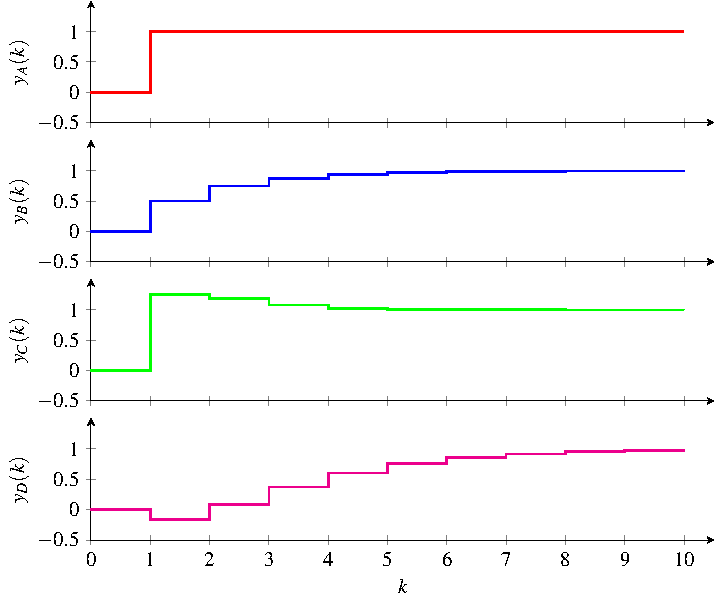
\includegraphics[width=0.50\columnwidth]{./Unit-04/img/StepRespTypes.pdf}
       \end{center}
 \item \vspace{-3mm} Let us try to provide some possible interpretation.
 \end{itemize}
\end{frame}

\begin{frame}
\frametitleTC{Generalisation}
\framesubtitleTC{One model class, different responses}
\myPause
 \begin{columns}
  \column[T]{0.45\textwidth}
   \only<2->{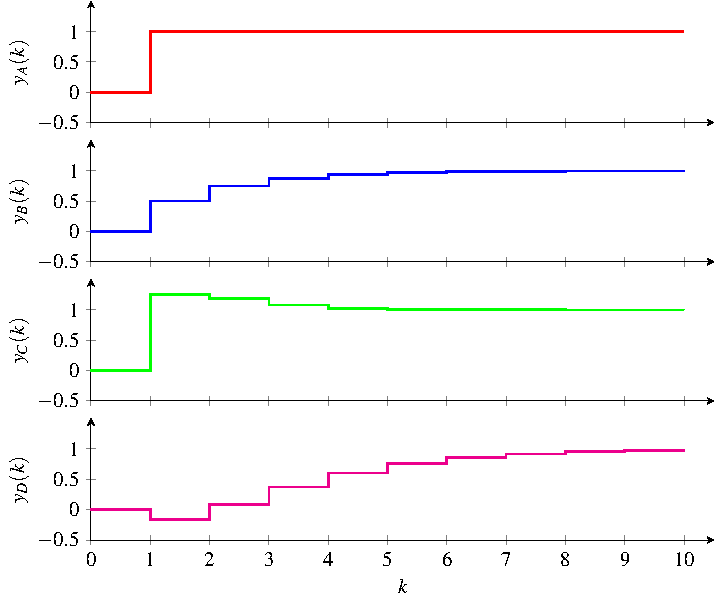
\includegraphics[height=5.5cm]{./Unit-04/img/StepRespTypes.pdf}}
  \column[T]{0.55\textwidth}
   \begin{itemize}[<+-| alert@+>]
   \item Suppose $u(k)$ and $y(k)$ to be respectively a resource to allot and its effect.
         \begin{itemize}[<+-| alert@+>]
         \item[A.] The resource is acquired and exerts immediately its effect (that is therefore
                   seen at the very next step).
         \item[B.] The resource acts immediately but takes some steps to yield its full effect\\
                   (for example because first\\
                   some queue needs\\
                   emptying).
         \end{itemize}
   \end{itemize}
 \end{columns}
\end{frame}

\begin{frame}
\frametitleTC{Generalisation}
\framesubtitleTC{One model class, different responses}
 \begin{columns}
  \column[T]{0.45\textwidth}
   \only<1->{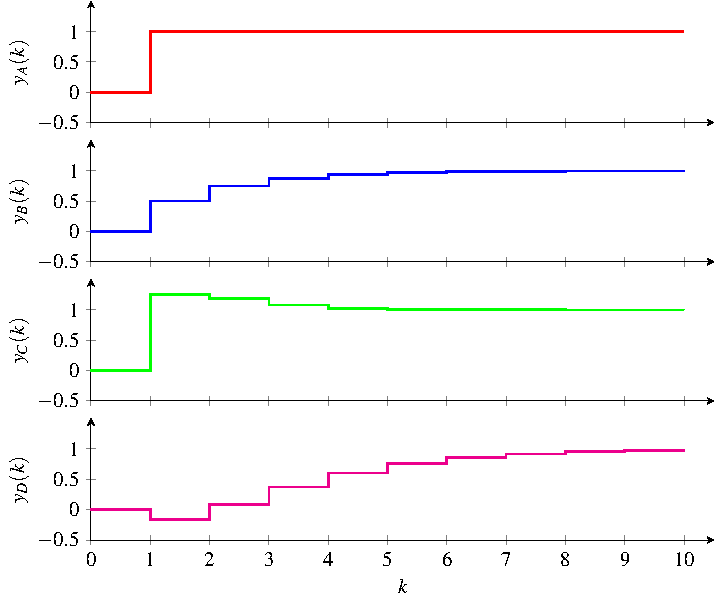
\includegraphics[height=5.5cm]{./Unit-04/img/StepRespTypes.pdf}}
  \column[T]{0.55\textwidth}
   \begin{itemize}[<+-| alert@+>]
   \item Suppose $u(k)$ and $y(k)$ to be respectively a resource to allot and its effect.
         \begin{itemize}[<+-| alert@+>]
         \item[C.] The resource produces a transiently enhanced effect (this is quite typical
                   when the resource is computational power and the effect is the \emph{speed} toward a goal).
         \item[D.] The resource requires some effort to be acquired and initially \emph{reduces}
                   performance, like a new\\
                   core that when acquired\\
                   has an unknown cache\\
                   content, thus causing\\
                   a lot of cache misses.
         \end{itemize}
   \end{itemize}
 \end{columns}
\end{frame}

\begin{frame}
\frametitleTC{Generalisation}
\framesubtitleTC{Lessons learnt and next steps}
\myPause
 \begin{itemize}[<+-| alert@+>]
 \item One model can produce very different responses \TC{by just changing parameters}, thus fitting
       several physical cases --- remember the remark in the introductory section, that we need a systems
       and control theory because determining a controller is largely physics-independent?.
 \item \vspace{3mm} We shall now see how control requirements can be stipulated by saying that some response
       to some \emph{stimulus} should have a certain aspect.
 \item We shall then convert this into requiring some \TC{transfer function}\\
       to have a certain aspect...
 \item ...and finally start synthesising feedback controllers.
 \end{itemize}
\end{frame}


\section{Formalising requirements}
\subsection{}

\begin{frame}
\frametitleTC{A time-domain viewpoint}
\framesubtitleTC{}
\myPause
 \begin{itemize}[<+-| alert@+>]
 \item Requirements are expressed in the time domain very naturally.
 \item Suppose to apply a step variation to the set point $w(k)$, and consider four possible\\
       responses of the controlled variable $y(k)$ --- points are joined with segments\\
       to improve readability:
       \begin{center}
        \vspace{2mm}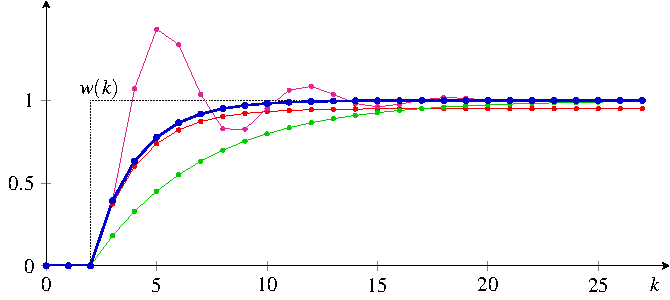
\includegraphics[width=0.60\columnwidth]{./Unit-04/img/StepRespForRequirements.pdf}
       \end{center}
 \end{itemize}
\end{frame}

\begin{frame}
\frametitleTC{A time-domain viewpoint}
\framesubtitleTC{}
\myPause
 \begin{center}
  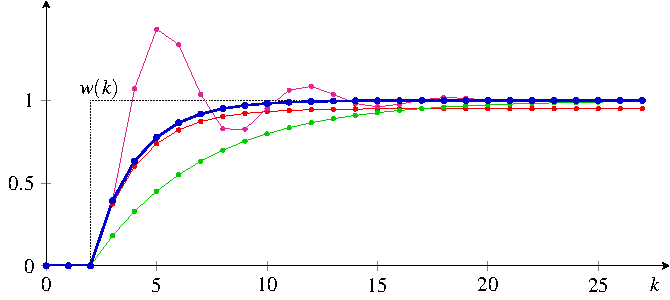
\includegraphics[width=0.40\columnwidth]{./Unit-04/img/StepRespForRequirements.pdf}
 \end{center}\myPause
 \begin{itemize}[<+-| alert@+>]
 \item The ``control quality'' (for the moment, in the most intuitive sense)\\
       is different:
       \begin{itemize}[<+-| alert@+>]
       \item \textcolor{blue!80!black}{blue} -- good;
       \item \textcolor{red!95!black}{red} -- does not reach the new desired value exactly;
       \item \textcolor{green!80!black}{green} -- too slow;
       \item \textcolor{magenta!95!black}{magenta} -- oscillatory.
       \end{itemize}
 \end{itemize}
\end{frame}

\begin{frame}
\frametitleTC{A time-domain viewpoint}
\framesubtitleTC{}
\myPause
 \begin{itemize}[<+-| alert@+>]
 \item Indeed, many requirements are straightforwardly expressed by stating e.g. how the response
       of the controlled variable to a certain variation of the set point has to look.
 \item For example, one may require that
       \begin{itemize}[<+-| alert@+>]
       \item[] when $w(k)$ undergoes a step variation
       \item[] $y(k)$ has to enter a $\mp$5\% band around it in maximum 5 steps
       \item[] and then never exit that band,
       \item[] also never reaching a value more than 10\% above the new set point,
       \item[] and with a one-step variation not greater than half of the total one,
       \end{itemize}
 \item[] or express analogous desires.
 \end{itemize}
\end{frame}

\begin{frame}
\frametitleTC{A time-domain viewpoint}
\framesubtitleTC{}
\myPause
 \begin{itemize}[<+-| alert@+>]
 \item A quite articulated example to illustrate the idea is shown below: the response has to lie
       entirely within the evidenced area.
       \begin{center}
        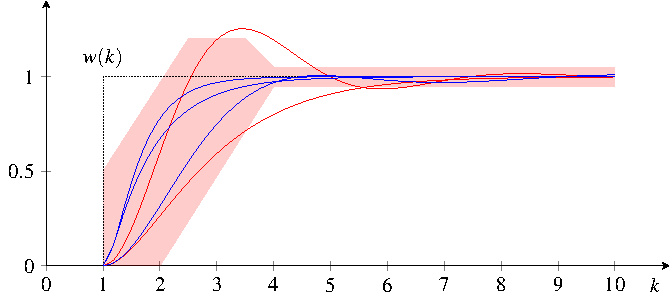
\includegraphics[width=0.60\columnwidth]{./Unit-04/img/StepRespWithConstraints-SP.pdf}
       \end{center}
 \item Blue responses are acceptable, red ones are not.
 \end{itemize}
\end{frame}


\begin{frame}
\frametitleTC{A time-domain viewpoint}
\framesubtitleTC{}
\myPause
 \begin{itemize}[<+-| alert@+>]
 \item The key idea we are soon introducing is that prescribing a certain aspect for the response
       of $y(k)$ to $w(k)$, in fact means prescribing characteristics of the transfer function
       from the former to the latter (as already anticipated).
 \item The same idea can be applied to the responses of $y(k)$ to disturbances, if the issue is to
       reject them.
 \item \vspace{3mm}This is not the only way to set requirements, but here we stick to this one.
 \item In the following we shall see how the idea above leads to synthesising\\
       a suitable controller --- and the PID structure will come into play\\
       \TC{with consciousness of the reasons for its wide applicability}.
 \item \vfill But prior to this, also to understand what a reasonable ``desired $y/w$\\
       transfer function'' can look like, we need to analyse the control loop\\
       formally.
 \end{itemize}
\end{frame}

\section{The control loop}
\subsection{}

\begin{frame}
\frametitleTC{The control loop and its actors}
\framesubtitleTC{}
\myPause
 \begin{itemize}[<+-| alert@+>]
 \item General representation:
       \begin{center}
        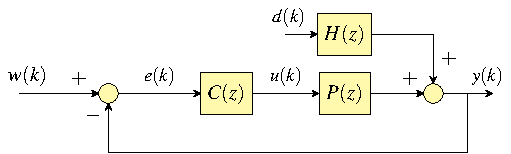
\includegraphics[width=0.50\columnwidth]{./Unit-04/img/ControlLoop.pdf}
       \end{center}
 \item Notation:
       \begin{itemize}[<+-| alert@+>]
       \item $w(k)$ is the \TC{set point} or \TC{reference};
       \item $y(k)$ is the \TC{controlled variable};
       \item $e(k)$ is the \TC{error};
       \item $u(k)$ is the \TC{control signal};
       \item $d(k)$ is a \TC{disturbance};
       \item $P(z)$ and $H(z)$ compose the \TC{controlled system} model;
       \item $C(z)$ is the \TC{controller} transfer function.
       \end{itemize}
 \end{itemize}
\end{frame}

\begin{frame}
\frametitleTC{The control loop and its actors}
\framesubtitleTC{}
 \begin{center}
  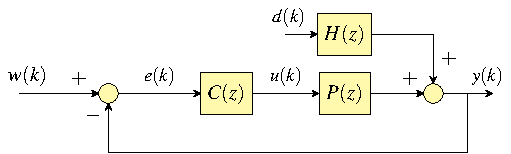
\includegraphics[width=0.40\columnwidth]{./Unit-04/img/ControlLoop.pdf}
 \end{center}
 \begin{itemize}[<+-| alert@+>]
 \item \vspace{-2mm} Some remarks:
       \begin{itemize}[<+-| alert@+>]
       \item we assume that the \TC{measurement} of $y$ reaching the node that generates the error,
             is exact (no disturbance on the feedback line) and instantaneous (no dynamic block
             on that line either);
       \item this may be \emph{very} questionable when some sensor is in the \emph{arena}, thus for\\
             example is not always assumed in process control, robotics and the like;
       \item however in computers most measurements are in fact the measured\\
             quantity itself (e.g., the one timer firing preemption interrupts and\\
             accounting CPU usage);
       \item this is an important simplification to exploit when applying control\\
             to computing system,
       \item with the exception of more ``physical'' controls (temperature, power,...)\\
             where sensor dynamics may be of some concern.
       \end{itemize}
 \end{itemize}
\end{frame}

\begin{frame}
\frametitleTC{Intermezzo}
\framesubtitleTC{Composing blocks in a feedback structure (we still miss this besides series and parallel)}
 \begin{center}
  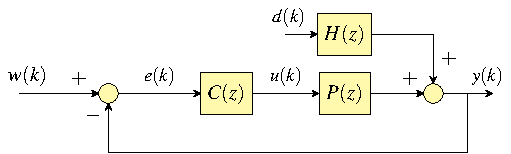
\includegraphics[width=0.40\columnwidth]{./Unit-04/img/ControlLoop.pdf}
 \end{center}\myPause
 \begin{itemize}[<+-| alert@+>]
 \item We need to compute the transfer functions from $w$ and $d$ to $y$ and $u$.
 \item To this end, imagine to cut the loop (for example right of the node summing the outputs of $P$ and $H$).
 \item Equating the left and the right side of this fictitious cut we have
       \begin{displaymath}
        H(z)d(k) + P(z)C(z) \left(w(k)-y(k) \right) = y(k),
       \end{displaymath}
 \item whence rearranging
       \begin{displaymath}
        y(k) = \frac{P(z)C(z)}{1+P(z)C(z)} w(k) + \frac{H(z)}{1+P(z)C(z)} d(k).
       \end{displaymath}
 \end{itemize}
\end{frame}

\begin{frame}
\frametitleTC{Intermezzo}
\framesubtitleTC{Composing blocks in a feedback structure}
\myPause
 \begin{itemize}[<+-| alert@+>]
 \item We adopt from now on the convention of calling $G_{ba}(z)$ the transfer function from $a(k)$ to $b(k)$
       when convenient --- btw, mind the subscript order. 
 \item We also recall the operatorial meaning of a transfer function, and that it represents the \TC{effect}
       of a certain input to a certain output. In other words, in our case we should for completeness write
       \begin{displaymath}
        G_{yw}(z) = \left. \frac{y(k)}{w(k)} \right|_{d(k)=0}, \qquad
        G_{yd}(z) = \left. \frac{y(k)}{d(k)} \right|_{w(k)=0},
       \end{displaymath}
       but we drop part of the notation for simplicity.
 \item Summing up, we have
       \begin{displaymath}
        G_{yw}(z) = \frac{P(z)C(z)}{1+P(z)C(z)}, \qquad
        G_{yd}(z) = \frac{H(z)}{1+P(z)C(z)}.
       \end{displaymath}
 \end{itemize}
\end{frame}

\begin{frame}
\frametitleTC{Intermezzo}
\framesubtitleTC{Composing blocks in a feedback structure}
\myPause
 \begin{center}
  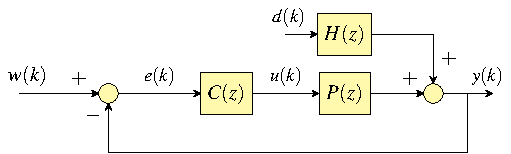
\includegraphics[width=0.40\columnwidth]{./Unit-04/img/ControlLoop.pdf}
 \end{center}\myPause
 \begin{itemize}[<+-| alert@+>]
 \item Reasoning in the same way for the output $u(k)$ -- details left as an exercise -- we have
       \begin{displaymath}
        G_{uw}(z) =  \frac{C(z)}{1+P(z)C(z)}, \qquad
        G_{ud}(z) = -\frac{C(z)H(z)}{1+P(z)C(z)}.
       \end{displaymath}
 \end{itemize}
\end{frame}

\begin{frame}
\frametitleTC{The control loop and its actors}
\framesubtitleTC{Main transfer functions of interest}
\myPause
 \begin{itemize}[<+-| alert@+>]
 \item Loop:
       \begin{displaymath}
        L(z) := P(z)C(z).
       \end{displaymath}
 \item From set point to controlled variable and control signal:
       \begin{displaymath}
        G_{yw}(z) = \frac{L(z)}{1+L(z)}, \qquad
        G_{uw}(z) = \frac{C(z)}{1+L(z)}.
       \end{displaymath}
 \item From disturbance to controlled variable and control signal:
       \begin{displaymath}
        G_{yd}(z) =  \frac{H(z)}{1+L(z)}, \qquad
        G_{ud}(z) = -\frac{C(z)H(z)}{1+L(z)}.
       \end{displaymath}
 \end{itemize}
\end{frame}

\begin{frame}
\frametitleTC{The control part of the loop}
\framesubtitleTC{Functional view}
\myPause
 \begin{itemize}[<+-| alert@+>]
 \item For the loop to operate
       \begin{itemize}[<+-| alert@+>]
       \item an \TC{event generator} triggers a new control action (periodically or on demand,\\
             here we stick to the former case);
       \item a \TC{sensor} is activated to get $y(k)$;
       \item the \TC{controller} $C(z)$ is invoked, and evolves as dynamic system by one step,
             \begin{itemize}[<+-| alert@+>]
             \item updating its state
             \item and then computing the new control $u(k)$;
             \end{itemize}
       \item an \TC{actuator} is activated to act on the process;
       \item and finally the system waits for a new event.
       \end{itemize}
 \item \vfill This view is quite easily related to CS frameworks such as\\
       the MAPE(-K).
 \item However, to design the controller, another view is preferable.
 \end{itemize}
\end{frame}

\begin{frame}
\frametitleTC{The control part of the loop}
\framesubtitleTC{Systemic view}
\myPause
 \begin{itemize}[<+-| alert@+>]
 \item For the loop to operate correctly
       \begin{itemize}[<+-| alert@+>]
       \item the closed-loop system must be asymptotically stable (more detail on this matter coming soon);
       \item the reference-to-output transfer function $G_{yw}(z)$, and/or the disturbance-to-output one $G_{yd}(z)$,
             must yield ``acceptable'' time responses in the presence of \TC{expectable} signals $w(k)$ and $d(k)$;
       \item the controller must be \TC{realisable}, i.e., the order of the numerator of $C(z)$ cannot exceed
             that of the denominator;
       \item in the opposite case, to explain the term ``realisable'', the controller\\
             output would depend on FUTURE samples of its input, which clearly\\ 
             is impossible to realise.
       \item We already saw that the above degree relationship is a structural\\
             property of any properly defined transfer function, incidentally.
       \end{itemize}
 \end{itemize}
\end{frame}

\begin{frame}\mccz
\frametitleTC{Time to start assembling our puzzle}
\framesubtitleTC{}
\myPause
 \begin{columns}
  \column[T]{0.35\textwidth}
   \only<2->{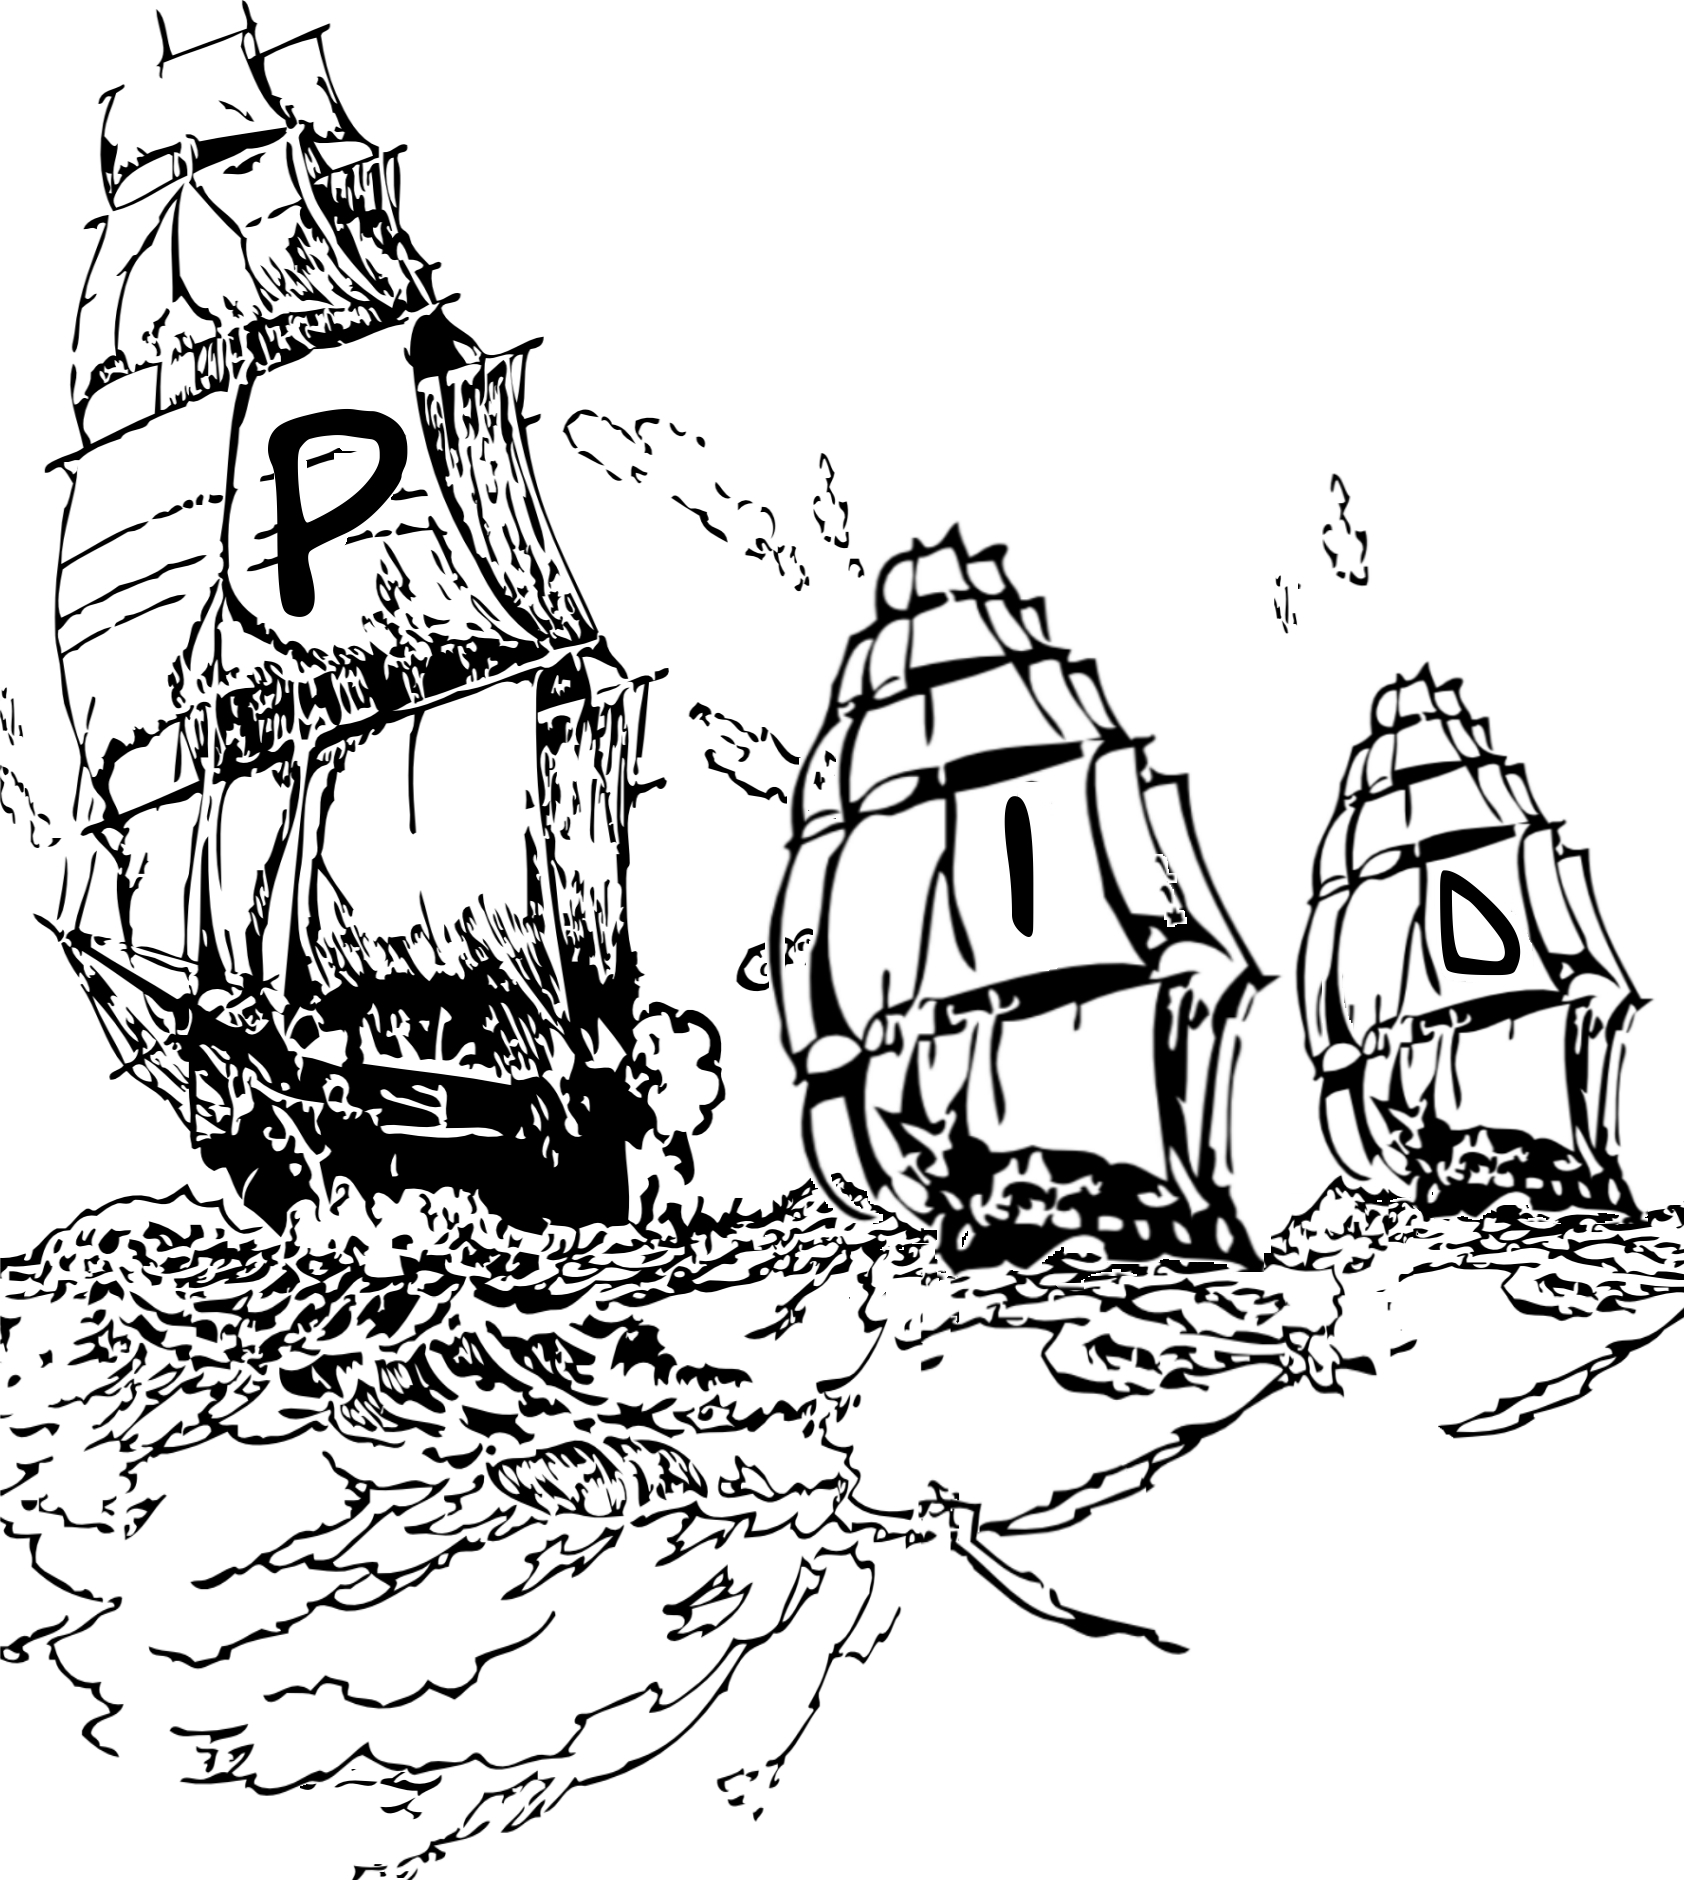
\includegraphics[height=6cm]{./Unit-04/img/PIDsOnTheHorizon_cc0.jpg}}
  \column[T]{0.65\textwidth}
   \begin{itemize}[<+-| alert@+>]
   \item First we shall learn a feedback control synthesis\\
         technique named ``direct'',
   \item then we shall discuss the relationships between\\
         the dynamic structure of the process\\
         and that of the controller,
   \item finally coming, as a quite natural\\
         consequence, to anticipate\\
         the PID control law. 
   \end{itemize}
 \end{columns}
\end{frame}



\section{Direct synthesis}
\subsection{}

\begin{frame}
\frametitleTC{Introductory example}
\framesubtitleTC{as usual...}
\myPause
 \begin{itemize}[<+-| alert@+>]
 \item Consider the control loop we know, with $H(z)=1$ for simplicity:
       \begin{center}
        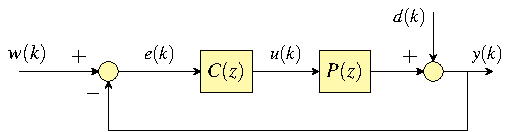
\includegraphics[width=0.50\columnwidth]{./Unit-04/img/ControlLoop-H1.pdf}
       \end{center}
 \item Take as process and controller, respectively,
       \begin{displaymath}
        P(z) = \frac{\mu}{z-p}, \qquad
        C(z) = \frac{1-\alpha}{\mu} \, \frac{z-p}{z-1},
       \end{displaymath}
 \item and analyse the obtained system.
 \end{itemize}
\end{frame}

\begin{frame}
\frametitleTC{Introductory example}
\framesubtitleTC{}
\myPause
 \begin{itemize}[<+-| alert@+>]
 \item We have a \TC{zero/pole cancellation} between controller and process, as the loop transfer function is
       \begin{displaymath}
        L(z) = P(z)C(z)
             = \frac{\cbcancel[gray]{\mu}}{\ccancel[red]{z-p}} \,
               \frac{1-\alpha}{\cbcancel[gray]{\mu}} \, \frac{\ccancel[red]{z-p}}{z-1}
             = \frac{1-\alpha}{z-1}
       \end{displaymath}
 \item Hence
       \begin{displaymath}
        G_{yw}(z) = \frac{L(z)}{1+L(z)}
                  = \frac{\frac{1-\alpha}{z-1}}{1+\frac{1-\alpha}{z-1}}
                  = \frac{1-\alpha}{\ccancel[green!80!black]{z-1}} \,
                    \frac{\ccancel[green!80!black]{z-1}}{z-1+1-\alpha}
                  = \frac{1-\alpha}{z-\alpha}.
       \end{displaymath}
 \item NOTE: the \textcolor{green!80!black}{simplification} in computing $G_{yw}$ is NOT a cancellation.
 \item[] \vspace{-0.75mm}To have a cancellation you need a system (block) with a zero say\\
       in $\overline{z}$, and \TC{\underline{ANOTHER}} system (block) with a pole in the same  $\overline{z}$\\
 \item[] \vspace{-0.75mm} --- as is the case with the \textcolor{red}{cancellation} in $L$ above.
 \end{itemize}
\end{frame}

\begin{frame}
\frametitleTC{Introductory example}
\framesubtitleTC{}
\myPause
 \begin{itemize}[<+-| alert@+>]
 \item Furthermore, as $H(z)=1$,
       \begin{displaymath}
        G_{yd}(z) = \frac{1}{1+L(z)}
                  = \frac{1}{1+\frac{1-\alpha}{z-1}}
                  = \frac{z-1}{z-1+1-\alpha}
                  = \frac{z-1}{z-\alpha}.
       \end{displaymath}
 \item You may -- should \smiley$\,$ -- remember that cancellations entail hidden parts for the affected system.
 \item Let us evidence and discuss the implications of this in the present\\
       case, by going through a state space analysis.
 \end{itemize}
\end{frame}

\begin{frame}
\frametitleTC{Introductory example}
\framesubtitleTC{State space formulation of the closed-loop system}
\myPause
 \begin{itemize}[<+-| alert@+>]
 \item First we express the process in state space form:
       \begin{displaymath}
        \left\{\begin{array}{rcl}
         x_P(k) &=& p x_P(k-1) + \mu u(k-1) \\
         y(k)   &=& x_P(k) + d(k)
        \end{array}\right.
       \end{displaymath}
 \item Then we rewrite the controller transfer function as a constant plus a term with numerator degree
       strictly less than denominator degree (check out the wxMaxima \texttt{divide} function):
       \begin{displaymath}
        C(z) = \frac{1-\alpha}{\mu} \, \frac{z-p}{z-1} 
             = \frac{1-\alpha}{\mu} \left( 1 + \textcolor{red}{\frac{1-p}{z-1}} \right)
       \end{displaymath}
 \item Then we treat the \textcolor{red}{strictly proper} term like $P(z)$ above, obtaining
       \begin{displaymath}
        \left\{\begin{array}{rcl}
         x_C(k) &=& x_C(k-1) + (1-p) e(k-1) \\
         u(k)   &=& \frac{1-\alpha}{\mu} x_C(k) + \frac{1-\alpha}{\mu} e(k)
        \end{array}\right.
       \end{displaymath}
 \end{itemize}
\end{frame}

\begin{frame}
\frametitleTC{Introductory example}
\framesubtitleTC{State space formulation of the closed-loop system}
\myPause
 \begin{itemize}[<+-| alert@+>]
 \item Joining the equations for $P$ and $C$ and those for the node that produces $e$, gives\\
       for the overall closed-loop system the scalar (not yet reduced to minimal) description
       \begin{displaymath}
        \left\{\begin{array}{rcl}
         x_P(k) &=& p x_P(k-1) + \mu u(k-1) \\
         x_C(k) &=& x_C(k-1) + (1-p) e(k-1) \\
         y(k)   &=& x_P(k) + d(k) \\
         u(k)   &=& \frac{1-\alpha}{\mu} x_C(k) + \frac{1-\alpha}{\mu} e(k) \\
         e(k)   &=& w(k) - y(k)
        \end{array}\right.
       \end{displaymath}
 \end{itemize}
\end{frame}

\begin{frame}
\frametitleTC{Introductory example}
\framesubtitleTC{State space formulation of the closed-loop system}
\myPause
 \begin{itemize}[<+-| alert@+>]
 \item For the process state we have
       \begin{displaymath}
        \begin{array}{rcl}
         x_P(k) &=& p x_P(k-1) + \mu u(k-1) \\
                &=& p x_P(k-1) + \mu \left( \frac{1-\alpha}{\mu} x_C(k-1) + \frac{1-\alpha}{\mu} e(k-1) \right) \\
                &=& p x_P(k-1) + (1-\alpha)x_C(k-1) + (1-\alpha) \left( w(k-1)-y(k-1) \right) \\
                &=& p x_P(k-1) + (1-\alpha)x_C(k-1) + (1-\alpha) w(k-1)\\
                & & - (1-\alpha) \left( x_P(k-1)+d(k-1) \right) \\
                &=& \left( p+\alpha-1 \right) x_P(k-1)
                    +(1-\alpha) x_C(k-1)\\
                & & +(1-\alpha) w(k-1)
                    -(1-\alpha) d(k-1)                 
        \end{array}
       \end{displaymath}
 \item while the controller state evolves according to
       \begin{displaymath}
        \begin{array}{rcl}
         x_C(k) &=& x_C(k-1) + (1-p) e(k-1) \\
                &=& x_C(k-1)\\
                & & + (1-p) \left( w(k-1)-x_P(k-1)-d(k-1) \right)\\
                &=& (p-1) x_P(k-1) + x_C(k-1)\\
                & & +(1-p) w(k-1)
                    -(1-p) d(k-1)  
        \end{array}
       \end{displaymath}
 \end{itemize}
\end{frame}

\begin{frame}
\frametitleTC{Introductory example}
\framesubtitleTC{State space formulation of the closed-loop system}
\myPause
 \begin{itemize}[<+-| alert@+>]
 \item Putting it all together, the closed-loop system in state space form reads
       \begin{displaymath}
        \left\{\begin{array}{rcl}
         \begin{bmatrix} x_P(k) \\ x_C(k) \end{bmatrix}
         &=& 
         \begin{bmatrix} p+\alpha-1 & 1-\alpha \\ p-1 & 1  \end{bmatrix}
         \begin{bmatrix} x_P(k-1) \\ x_C(k-1) \end{bmatrix}
         +
         \begin{bmatrix} 1-\alpha & \alpha-1 \\ 1-p & p-1  \end{bmatrix}
         \begin{bmatrix} w(k-1) \\ d(k-1) \end{bmatrix} \\
         \begin{bmatrix} y(k) \\ u(k) \end{bmatrix}
         &=& 
         \begin{bmatrix} 1 & 0 \\ \frac{\alpha-1}{\mu} & \frac{1-\alpha}{\mu} \end{bmatrix}
         \begin{bmatrix} x_P(k) \\ x_C(k) \end{bmatrix}
         +
         \begin{bmatrix} 0 & 1 \\ \frac{1-\alpha}{\mu} & \frac{\alpha-1}{\mu} \end{bmatrix}
         \begin{bmatrix} w(k) \\ d(k) \end{bmatrix} \\
        \end{array}\right.
       \end{displaymath}
 \item[] with input $[w\,d]'$, output $[y\,u]'$ and
       \begin{displaymath}
        \begin{array}{c}
         A = \begin{bmatrix} p+\alpha-1 & 1-\alpha \\ p-1 & 1  \end{bmatrix},\quad
         B = \begin{bmatrix} 1-\alpha & \alpha-1 \\ 1-p & p-1  \end{bmatrix},\\
         C = \begin{bmatrix} 1 & 0 \\ \frac{\alpha-1}{\mu} & \frac{1-\alpha}{\mu} \end{bmatrix},\quad
         D = \begin{bmatrix} 0 & 1 \\ \frac{1-\alpha}{\mu} & \frac{\alpha-1}{\mu} \end{bmatrix}.
        \end{array}
       \end{displaymath}
 \end{itemize}
\end{frame}

\begin{frame}[fragile]
\frametitleTC{Introductory example}
\framesubtitleTC{State space formulation of the closed-loop system}
\myPause
 \begin{itemize}[<+-| alert@+>]
 \item To verify, we express the same system as a \TC{transfer matrix}, i.e.
       \begin{displaymath}
        \begin{bmatrix} y(k) \\ u(k) \end{bmatrix}
        = G(z) 
        \begin{bmatrix} w(k) \\ d(k) \end{bmatrix}, \qquad
        G(z) =
        \begin{bmatrix} G_{yw}(z) & G_{yd}(z) \\ G_{uw}(z) & G_{ud}(z) \end{bmatrix}
       \end{displaymath}
 \item Since $G(z) = C(zI-A)^{-1}B+D$, we can compute it in wxMaxima with 
       \begin{verbatim}
A : matrix([p+alpha-1,1-alpha],[p-1,1]);
B : matrix([1-alpha,alpha-1],[1-p,p-1]);
C : matrix([1,0],[(alpha-1)/mu,(1-alpha)/mu]);
D : matrix([0,1],[(1-alpha)/mu,(alpha-1)/mu]);
G : factor(C.invert(z*ident(2)-A).B+D);
       \end{verbatim}
 \end{itemize}
\end{frame}

\begin{frame}
\frametitleTC{Introductory example}
\framesubtitleTC{State space formulation of the closed-loop system}
\myPause
 \begin{itemize}[<+-| alert@+>]
 \item Doing so we obtain
       \begin{displaymath}
        G(z) =
        \begin{bmatrix} 
         \cfrac{1-\alpha}{z-\alpha}                   & \cfrac{z-1}{z-\alpha} \\
         \cfrac{1-\alpha}{\mu}\,\cfrac{z-p}{z-\alpha} & \cfrac{\alpha-1}{\mu}\,\cfrac{z-p}{z-\alpha}
        \end{bmatrix}
       \end{displaymath}
 \item The first row contains the transfer functions we already computed.
 \item The second says that the effects of $w$ and $d$ on $u$ are the opposite\\
       of one another (consistent with the loop scheme).
 \item \vfill Now, for some remarks to generalise.
 \end{itemize}
\end{frame}

\begin{frame}
\frametitleTC{Remarks}
\framesubtitleTC{and lessons learnt (1/2)}
\myPause
 \begin{itemize}[<+-| alert@+>]
 \item We took a first-order process.
 \item We took a controller that cancels the process pole with its zero, and has\\
       a pole in $z=1$.
 \item We obtained a reference-to-output transfer function $G_{yw}(z)$
       \begin{itemize}[<+-| alert@+>]
       \item with unity gain, hence for constant $w$ the error vanishes,
       \item and with a prescribed pole $\alpha$ (i.e., a prescribed set point tracking speed).
       \end{itemize}
 \item We also obtained a disturbance-to-output transfer function $G_{yd}(z)$
       \begin{itemize}[<+-| alert@+>]
       \item with zero gain, hence for constant $d$ the error vanishes as well,
       \item and with the same pole $\alpha$ (i.e., a prescribed disturbance rejection\\
             speed as well).
       \end{itemize}
 \end{itemize}
\end{frame}

\begin{frame}
\frametitleTC{Remarks}
\framesubtitleTC{and lessons learnt (2/2)}
\myPause
 \begin{itemize}[<+-| alert@+>]
 \item Most important, the eigenvalues of the closed-loop dynamic matrix $A$\\
       are $\alpha$ and $p$, i.e., \TC{the one we prescribed and the one we cancelled}.
 \item The latter eigenvalue apparently ends up in a hidden part --- the transfer matrix
       contains elements with a denominator of degree one and root $p$, while the order\\
       of the system is two (one state variable for $P$ and one for $C$).
 \item Thus we can use this technique only if $|p|<1$, otherwise the\\
       closed-loop system has a hidden part that is not asymptotically stable.
 \item \vfill We are now ready to address the \TC{direct synthesis} technique\\
       in general, at the level we need for our activity.
 \end{itemize}
\end{frame}

\begin{frame}
\frametitleTC{Direct synthesis}
\framesubtitleTC{The general idea}
\myPause
 \begin{itemize}[<+-| alert@+>]
 \item Assume a process model $P(z)$ is available.
 \item Choose a closed-loop transfer function -- name it here generically $O(z)$, specialisations
       in the following -- to represent your control objectives.
 \item Choose a desired expression $O^{\circ}(z)$ for $O(z)$.
 \item Express $O$ as a function of $P$ and the controller $C$ and set it equal to $O^{\circ}$,\\
       i.e., write the equation
       \begin{displaymath} 
       O \left( P(z),C(z) \right) = O^{\circ}(z).
       \end{displaymath}
 \item Solve for $C(z)$. Voil\`{a} \smiley.
 \end{itemize}
\end{frame}

\begin{frame}
\frametitleTC{Direct synthesis}
\framesubtitleTC{The general idea}
\myPause
 \begin{itemize}[<+-| alert@+>]
 \item \emph{CAVEAT 1:} no exhaustiveness claim. We are only scratching the surface,\\
       there is a myriad of things we cannot stuff in this course. Categorised\\
       references for the interested at the end.
 \item \emph{CAVEAT 2:} no magic either. There is potential but also pitfalls\\
       to be aware of.
 \item Some facts we anticipate right from the start:
       \begin{itemize}[<+-| alert@+>]
       \item direct synthesis inherently involves zero/pole cancellations,
       \item and an improper choice of $O^{\circ}$ may give a non realisable controller,
       \item thus overall not all desired dynamics can be obtained.
       \end{itemize}
 \item \vfill An important by-product of a system-theoretical approach, is that\\
       such limits can be set and discussed objectively.
 \end{itemize}
\end{frame}

\begin{frame}
\frametitleTC{Direct synthesis for set point tracking}
\framesubtitleTC{}
\myPause
 \begin{center}
  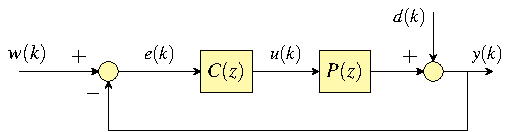
\includegraphics[width=0.50\columnwidth]{./Unit-04/img/ControlLoop-H1.pdf}
 \end{center}
 \begin{itemize}[<+-| alert@+>]
 \item The target transfer function is $G_{yw}(z)$, that we set equal to a desired $G_{yw}^{\circ}(z)$ writing
       \begin{displaymath} 
       \frac{P(z)C(z)}{1+P(z)C(z)} = G_{yw}^{\circ}(z).
       \end{displaymath}
 \item Solving for $C(z)$ we get
       \begin{displaymath} 
        C(z) = \frac{1}{P(z)} \, \frac{G_{yw}^{\circ}(z)}{1-G_{yw}^{\circ}(z)}.
       \end{displaymath}
 \item Note the cancellation (the $1/P$ factor in $C$).
 \end{itemize}
\end{frame}

\begin{frame}
\frametitleTC{Direct synthesis for disturbance rejection}
\framesubtitleTC{}
\myPause
 \begin{center}
  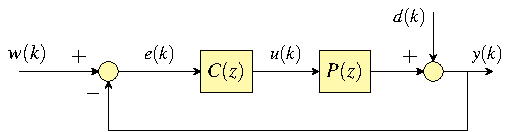
\includegraphics[width=0.50\columnwidth]{./Unit-04/img/ControlLoop-H1.pdf}
 \end{center}
 \begin{itemize}[<+-| alert@+>]
 \item The target transfer function is $G_{yd}(z)$, that we set equal to a desired $G_{yd}^{\circ}(z)$ writing
       \begin{displaymath} 
       \frac{1}{1+P(z)C(z)} = G_{yd}^{\circ}(z).
       \end{displaymath}
 \item Solving for $C(z)$ we get
       \begin{displaymath} 
        C(z) = \frac{1}{P(z)} \, \frac{1-G_{yd}^{\circ}(z)}{G_{yd}^{\circ}(z)}.
       \end{displaymath}
 \item Note the cancellation (the $1/P$ factor in $C$).
 \end{itemize}
\end{frame}

\begin{frame}\mccz
\frametitleTC{Direct synthesis}
\framesubtitleTC{Why ``PIDs on the horizon''?}
\myPause
 \begin{columns}
  \column[T]{0.35\textwidth}
   \only<2->{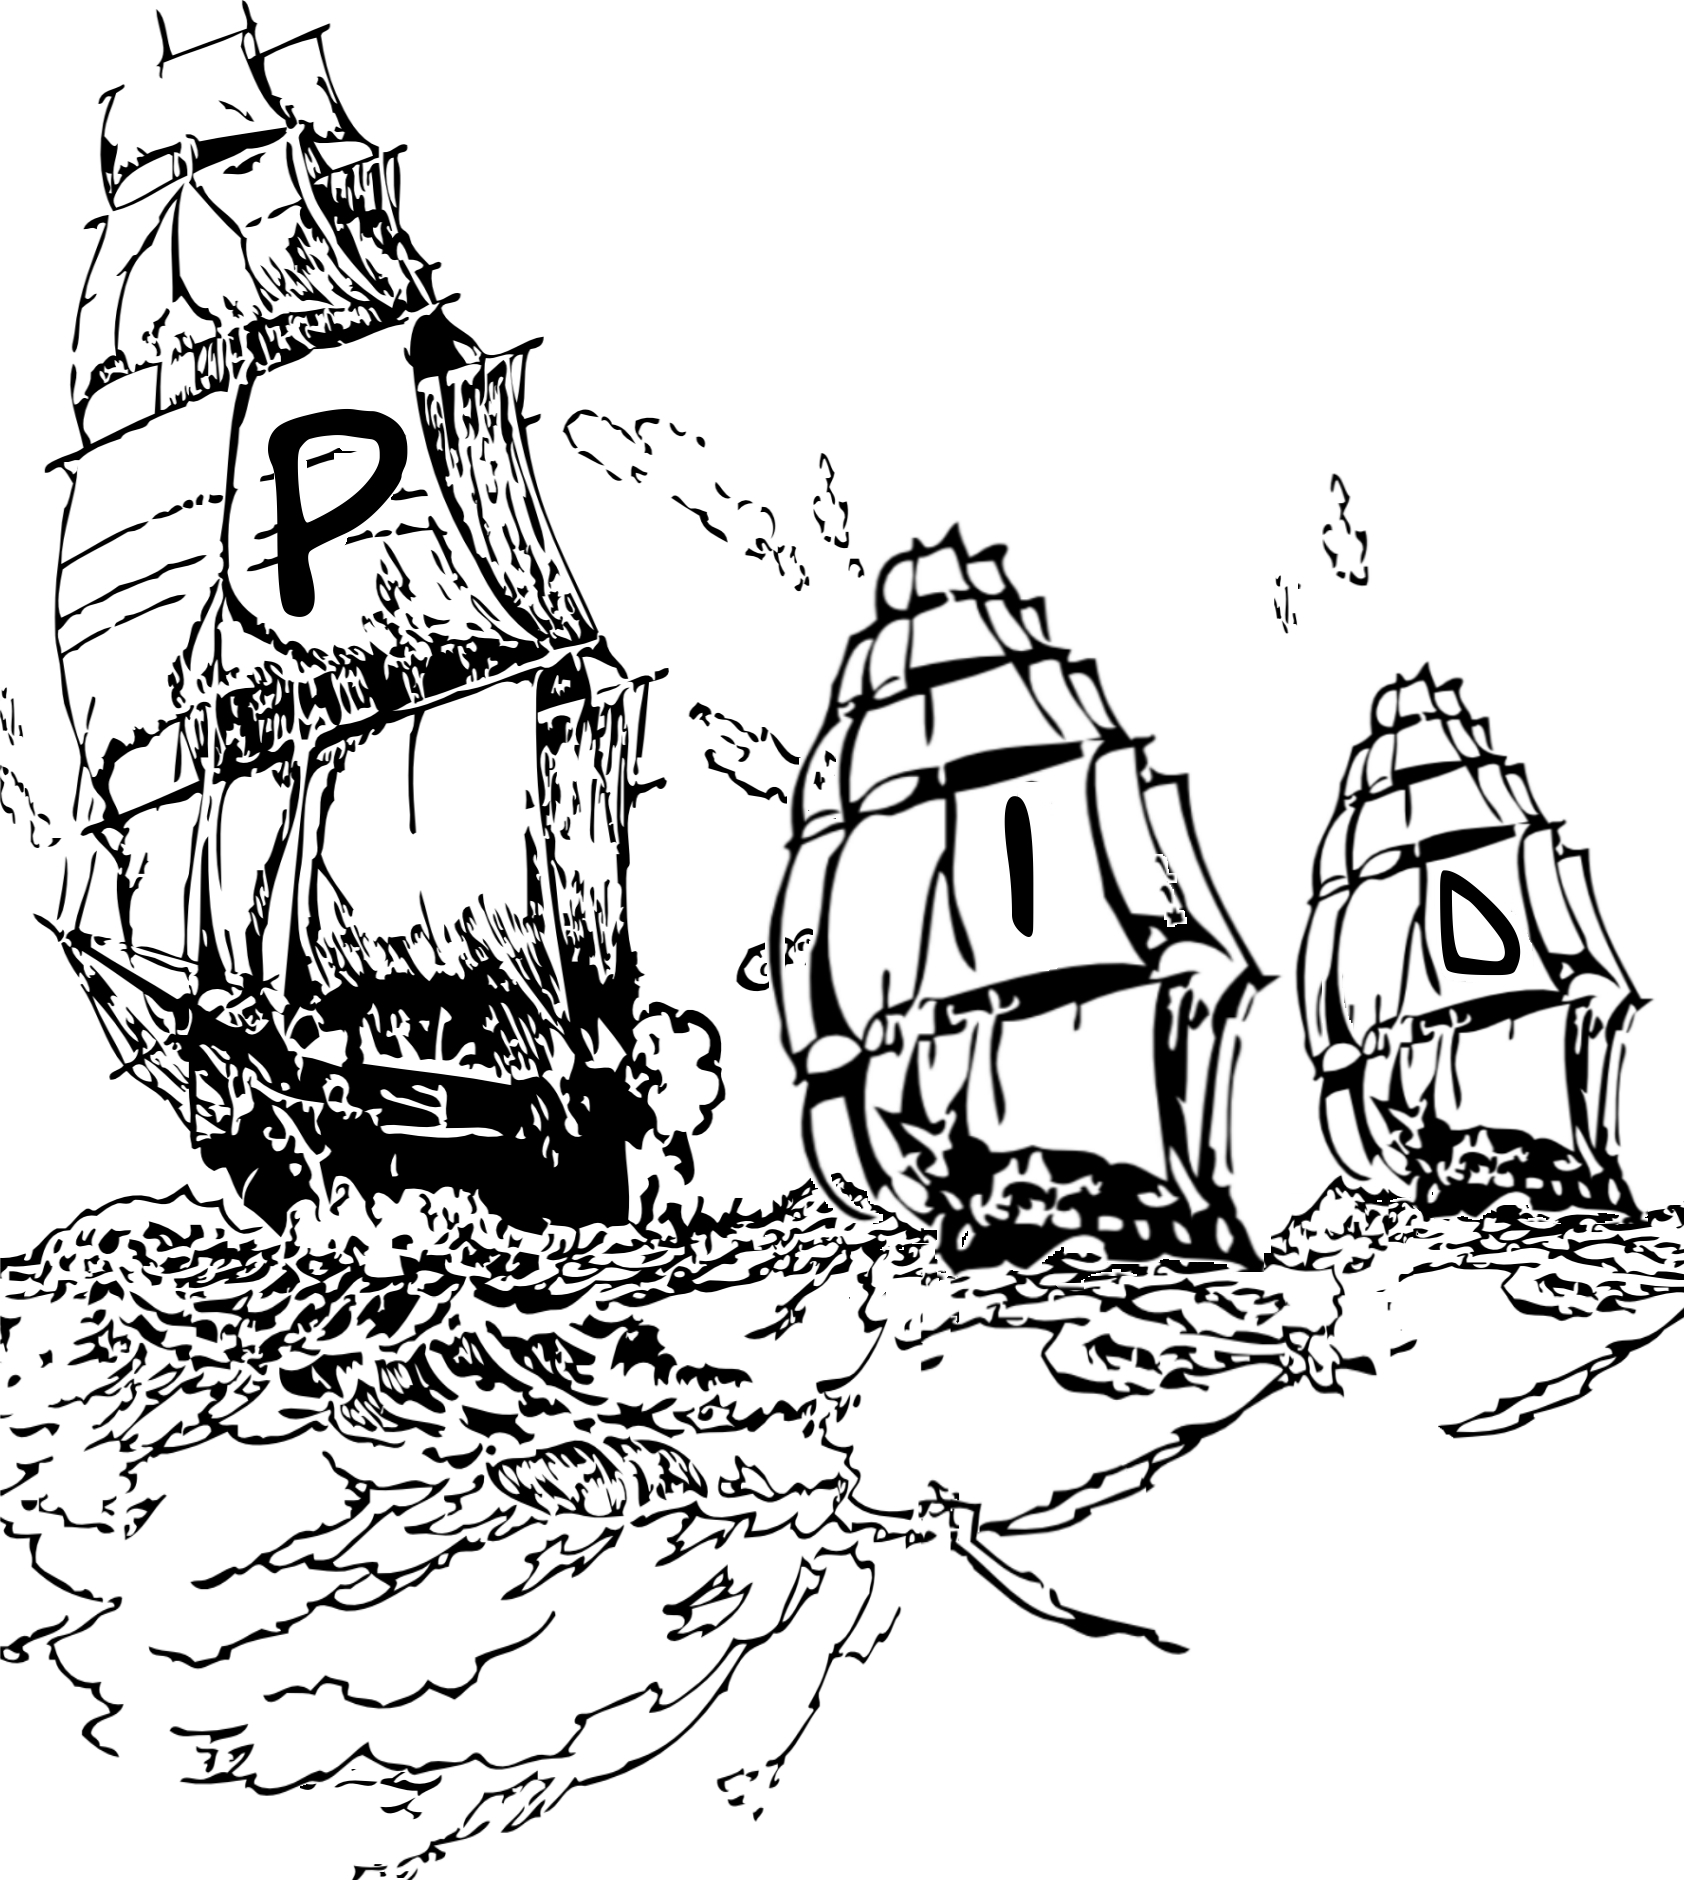
\includegraphics[height=6cm]{./Unit-04/img/PIDsOnTheHorizon_cc0.jpg}}
  \column[T]{0.65\textwidth}
   \begin{itemize}[<+-| alert@+>]
   \item Because applying direct synthesis to the versatile\\
         model we used to generate a variety of responses,\\
         with a sensible target transfer function, naturally\\
         leads to a controller with two zeroes and two\\
         poles, one of which in $z=1$.
   \item This is a PID controller.
   \item However we introduced a lot of material\\
         in this lecture.
   \item Better take a breath, recap, ad go\\
         through a practice session.
   \end{itemize}
 \end{columns}
\end{frame}





\section{Conclusions}
\subsection{}

\begin{frame}
\frametitleTC{Conclusions}
\framesubtitleTC{Recap and lessons learnt (1/2)}
\myPause
 \begin{itemize}[<+-| alert@+>]
 \item We can characerise a dynamic system with \TC{time domain responses}.
 \item These refer to a certain \emph{stimulus} (we used impulse and step).
 \item Responses can be used also to stipulate \TC{control objectives}.
 \item A viable way to do so is to transform time domain deires into some desired
       closed-loop transfer function.
 \item This paves the way to the \TC{direct synthesis} technique.
 \end{itemize}
\end{frame}

\begin{frame}
\frametitleTC{Conclusions}
\framesubtitleTC{Recap and lessons learnt (2/2)}
\myPause
 \begin{itemize}[<+-| alert@+>]
 \item We have open issues, however.
       \begin{itemize}[<+-| alert@+>]
       \item Why impulse and step \emph{stimuli} are meaningful?
       \item How can we choose the target closed-loop transfer function?
       \item What are the limits and what is their origin?
       \end{itemize}
 \item \vfill These issues are very suited for addressing in a practice session,\\
       which is our next task.
 \item Please review your notes, next time ask questions if needed\\
       before we start.
 \end{itemize}
\end{frame}

\section{}
{
\setbeamertemplate{headline}{
  \begin{beamercolorbox}[wd=\paperwidth,ht=4.2ex,dp=1.5ex]{palette quaternary}
  \end{beamercolorbox}
  }
\setbeamertemplate{footline}{
  \begin{beamercolorbox}[wd=\paperwidth,ht=2.2ex,dp=1.5ex]{palette quaternary}
  \end{beamercolorbox}
  }
\begin{frame}[noframenumbering]
 \vspace{20mm}\Huge{Discussion open}
\end{frame}
}


